\subsection{Inteligencia Artificial}
 Durante la conferencia de Darmouth en 1956, el informático John McCarthy introdujo por primera vez el término "Inteligencia Artificial" al mundo. McCarthy basó su concepto en los fundamentos teóricos publicados por Turing en 1950, donde se planteaba la posibilidad de que las máquinas pudieran pensar. En este evento, diversos investigadores y científicos expusieron los objetivos y la visión de la IA. Esta conferencia es ampliamente considerada como el punto de partida de la inteligencia artificial según se sabe en la actualidad. \parencite{teamredac2022}.
 Asimismo, hoy en día, no tenemos un concepto exacto acerca de la inteligencia artificial, debido a que es un tema complejo, por lo tanto, es posible hallar distintos conceptos acerca de ella. No obstante, la definición que se usará para términos de la investigación es que la inteligencia artificial es el poder de un ordenador de utilizar algoritmos, recibir datos, procesarlos y en base a esos pasos ser capaz de tomar decisiones similares a las de un ser humano. A diferencia de los humanos, la IA a través del procesamiento de conjuntos de información es capaz de crear máquinas y sistemas para resolver problemas que usualmente necesitan de inteligencia humana para resolverse. Muchos de los algoritmos de la IA se entrenan constituyéndose de datos para mejorar su rendimiento y optimizar las reglas establecidas, lo que se conoce como aprendizaje profundo \parencites{rouhiainen2018inteligencia}{ricardo2021inteligencia}{cajahuanca2021inteligencia}. 
 Por otro lado, hoy podemos encontrar diferentes tipos de IA, cada una con sus diferentes propósitos y características, de las más conocidas y aplicables en distintos campos académicos y profesionales, como la agricultura e ingeniería, son  Deep learning,  Vision Computer, este mismo contempla técnicas como Vision Transformer, Redes Neuronales Convolucionales, You Only Look One y técnicas para clasificación y regresión como Support Vector Machine.
 
 \subsection{Deep Learning}
 El Aprendizaje profundo, que particularmente se usa en los contextos donde la data es compleja y donde hay enormes cantidades de datos disponibles. Este subcampo de la inteligencia artificial se desarrolla mediante el uso de redes neuronales, las cuales se estructuran en niveles de procesamiento para identificar patrones y estructuras en conjuntos de datos extensos. Cada capa aprende un concepto de los datos sobre el que se basan las capas siguientes; cuanto más alto el nivel (capa), más abstractos son los conceptos aprendidos. El aprendizaje profundo no requiere un procesamiento previo de los datos y es capaz de extraer características de forma automática. Por poner una utilización sencilla, una red neuronal encargada de descifrar figuras aprendería a reconocer bordes simples en la primera capa y luego añadiría el reconocimiento de las figuras más complejas compuestas por esos bordes en las capas siguientes. No hay una regla fija sobre cuántas capas son necesarias para constituir una red neuronal profunda \parencites{rusk2016deep}{rouhiainen2018inteligencia}.
 Hoy en día muchas de las compañías online y grandes consumidoras de tecnología usan Inteligencia profunda. Por citar a una, Facebook usa esta tecnología para analizar los textos de las conversaciones. Otras compañías como Google, Baidu, y Microsoft usan inteligencia profunda para búsqueda de imágenes, y también traslación de máquinas. Todos los teléfonos inteligentes poseen sistemas de inteligencia profunda corriendo en ellos. Ahora, inteligencia profunda es el estándar para tecnología para reconocimiento del habla, y también para la detección de rostros por cámaras digitales. La inteligencia profunda, también es el centro de los autos que se manejan por sí mismos, donde es usual la localización y el mapeo, la percepción del entorno, planificación y dirección del movimiento, así como el seguimiento del estado del conductor. La inteligencia profunda está revolucionando la agricultura al proporcionar herramientas avanzadas para la clasificación y el análisis, lo que resulta en una mayor eficiencia, precisión y sostenibilidad en las prácticas agrícolas \parencite{kelleher2019deep}.
 
 \subsection{Vision Computer}
 Según \cite{alonso2016vision}, la Visión por computadora también conocido como visión artificial es otra rama importante de la IA que desempeña la tarea de dotar al computador la función de captar y comprender una imagen con el objetivo de emular el proceso que realizan los humanos. A pesar de tener menos tiempo a comparación con las otras, desempeña una función básica, primordial y compleja del reconocimiento. Esta es capaz de aprender y reconocer formas para luego darles una clasificación correctamente.
 Posee funciones como el reconocimiento donde en la imagen se indaga un objeto singular o reconocer diferentes instancias de una categoría genérica donde se hace dicho reconocimiento de la instancia. Este reconocimiento está asignado para categorizar diferentes clases a los objetos, el instrumento que ejecuta este procedimiento se llama clasificador.  Otro método es la representación de objetos, que se trata acerca de que los objetos sean identificados mediante segmentación de imágenes, pueden ser subdivididos en múltiples agrupaciones, desde el punto de agrupación, se provee de características comunes que tienen los objetos entre sí. El objeto medido según sus características es denominado patrón. Por último, tenemos al seguimiento de objetos en tiempo real, que consiste en que las técnicas o algoritmos de seguimiento estimen el movimiento de objetivo en el plano de la imagen mientras se da un contexto en movimiento, para eso el sistema coloca etiquetas fijas al objeto o los objetos a continuar durante continuidad de imágenes. La dificultad de esta técnica radica en los cambios inesperados en el movimiento, como la alteración en los aspectos de patrones, tal como de la escena, el propio objeto y las oclusiones entre objetos \parencite{alonso2016vision}.
 
 \subsection{Vision Transformer: Explainability of Vision Transformers: A Comprehensive Review and New Perspectives \citep*{tecnica1}}
 Los transformers han sido importantes en el procesamiento del lenguaje y, recientemente, se han destacado en la visión por computadora. Aunque su funcionamiento interno no se comprende completamente, la explicabilidad es crucial. Este estudio revisa métodos de explicabilidad para transformers visuales, propone una taxonomía y ofrece criterios de evaluación y herramientas. También señala áreas no exploradas que podrían mejorar la explicabilidad y sugiere futuras investigaciones.
 
 \subsubsection{Introducción}
 La Inteligencia Artificial (IA) ha experimentado avances notables en los últimos años, principalmente impulsada por el éxito de las Redes Neuronales Profundas (DNNs) en una amplia gama de aplicaciones, como el diagnóstico médico, las aplicaciones financieras, las evaluaciones de riesgos y la generación de imágenes y videos. Estos logros han sido significativos en términos de rendimiento y precisión en diversas tareas, sin embargo, la aplicación práctica de las DNNs sigue siendo limitada debido a su naturaleza opaca y la falta de transparencia en su toma de decisiones.
 
 La opacidad de las DNNs plantea preocupaciones importantes en términos de confiabilidad y seguridad, ya que los usuarios y los responsables de la toma de decisiones pueden tener dificultades para comprender por qué un modelo ha llegado a una determinada conclusión o recomendación. Esto es particularmente problemático en áreas donde las decisiones basadas en IA pueden tener un impacto significativo en la vida de las personas, como la salud y la justicia. La falta de transparencia también puede ocultar sesgos y errores en los modelos, lo que socava aún más la confianza en su uso.
 
 Para abordar estos desafíos, ha surgido el campo de la Inteligencia Artificial Explicable (XAI), cuyo objetivo es mejorar la comprensión y la transparencia de los modelos de IA. La XAI busca proporcionar explicaciones claras y comprensibles sobre cómo se toman las decisiones por parte de los modelos de IA, permitiendo a los usuarios entender y confiar en sus resultados. Al comprender cómo funciona un modelo y por qué toma ciertas decisiones, los usuarios pueden evaluar mejor su fiabilidad y corregir posibles sesgos o errores.
 
 En este contexto, los transformers, modelos basados en atención, han surgido como una alternativa poderosa a las arquitecturas de redes neuronales convolucionales (CNNs) tradicionales en áreas como el Procesamiento del Lenguaje Natural (NLP) y la Visión por Computadora (CV). Los transformers han demostrado ser altamente efectivos para capturar relaciones a largo plazo en datos secuenciales, lo que los hace adecuados para tareas que requieren un procesamiento de contexto complejo.
 
 En particular, los Vision Transformers (ViT) aplican la arquitectura de transformers a la tarea de visión por computadora, lo que ha llevado a avances significativos en tareas como el reconocimiento de imágenes, la detección de objetos y la segmentación de imágenes. Los ViT han demostrado resultados comparables e incluso superiores a los obtenidos con CNNs en algunas aplicaciones.
 
 Sin embargo, a pesar de su éxito, la comprensión y la explicabilidad de los transformers, especialmente en el contexto de la visión por computadora, siguen siendo áreas de investigación activa. Se necesitan métodos y técnicas robustas para explicar las decisiones tomadas por estos modelos, así como herramientas y marcos para evaluar y comparar sus explicaciones. Al mejorar la explicabilidad de los transformers, podemos fortalecer la confianza en su uso y abrir nuevas oportunidades para aplicaciones prácticas en una variedad de campos.
 
\subsubsection{ Arquitectura de Vision Transformer}
Los Vision Transformers (ViTs) aprovechan los avances de los transformers en NLP para aplicaciones visuales. Utilizan bloques de transformers que permiten integrar información global en toda la imagen mediante auto-atención. Las imágenes se representan como secuencias de tokens, con una capa de incrustación de parches para dividirlas en parches. Estos parches se aplanan y se tratan como tokens, luego se transforman en vectores de características. Para la clasificación, se agrega un token de clasificación. La red ViT también incluye otros componentes como una activación GELU, normalización de capa y conexión residual.Se puede encontrar una ilustración de la arquitectura ViT en la Figura 7.
  \begin{figure}[H]
  	\begin{center}
  		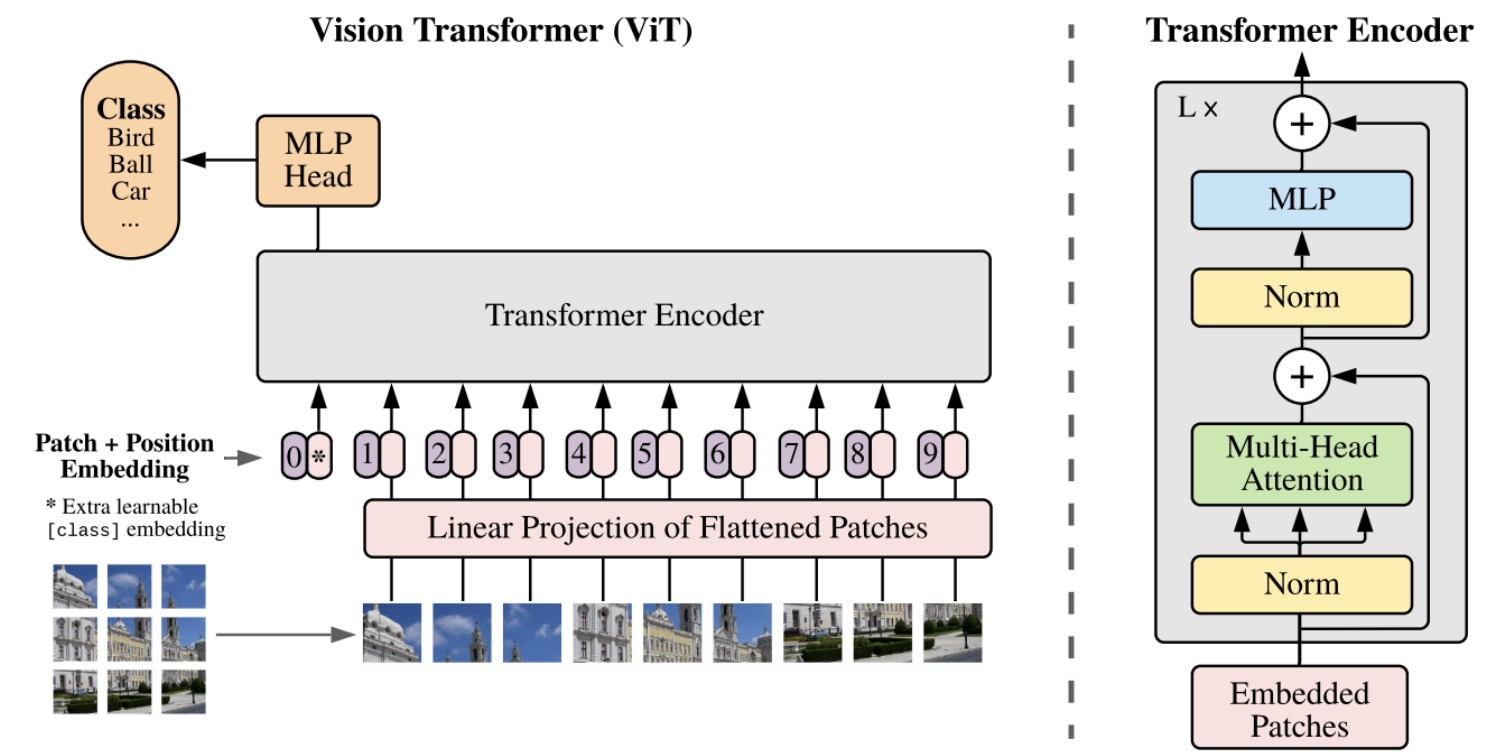
\includegraphics[width=1\textwidth]{2/figures/vt1.jpeg}
  		\caption{Arquitectura de Vision Transformer (\cite{tecnica1})}
  	\end{center}
  \end{figure}
 
 \subsubsection{ Explicacion y métodos para Visual Transformer} 
 Tras los trabajos innovadores presentados basados en transformers visuales para diversos dominios de visión por computadora, han surgido múltiples enfoques para mejorar la explicabilidad de estas redes. Sin embargo, se necesita una encuesta exhaustiva para comprender mejor estos métodos e identificar áreas de mejora. Con un enfoque en la tarea de clasificación, esta sección presenta una visión general de las técnicas de explicabilidad existentes para transformers visuales. Para proporcionar una visión clara, categorizamos y resumimos estos métodos en cinco grupos distintos según sus procedimientos de trabajo, motivaciones y características estructurales, como se ilustra en la Figura 8.
    \begin{figure}[H]
  	\begin{center}
  		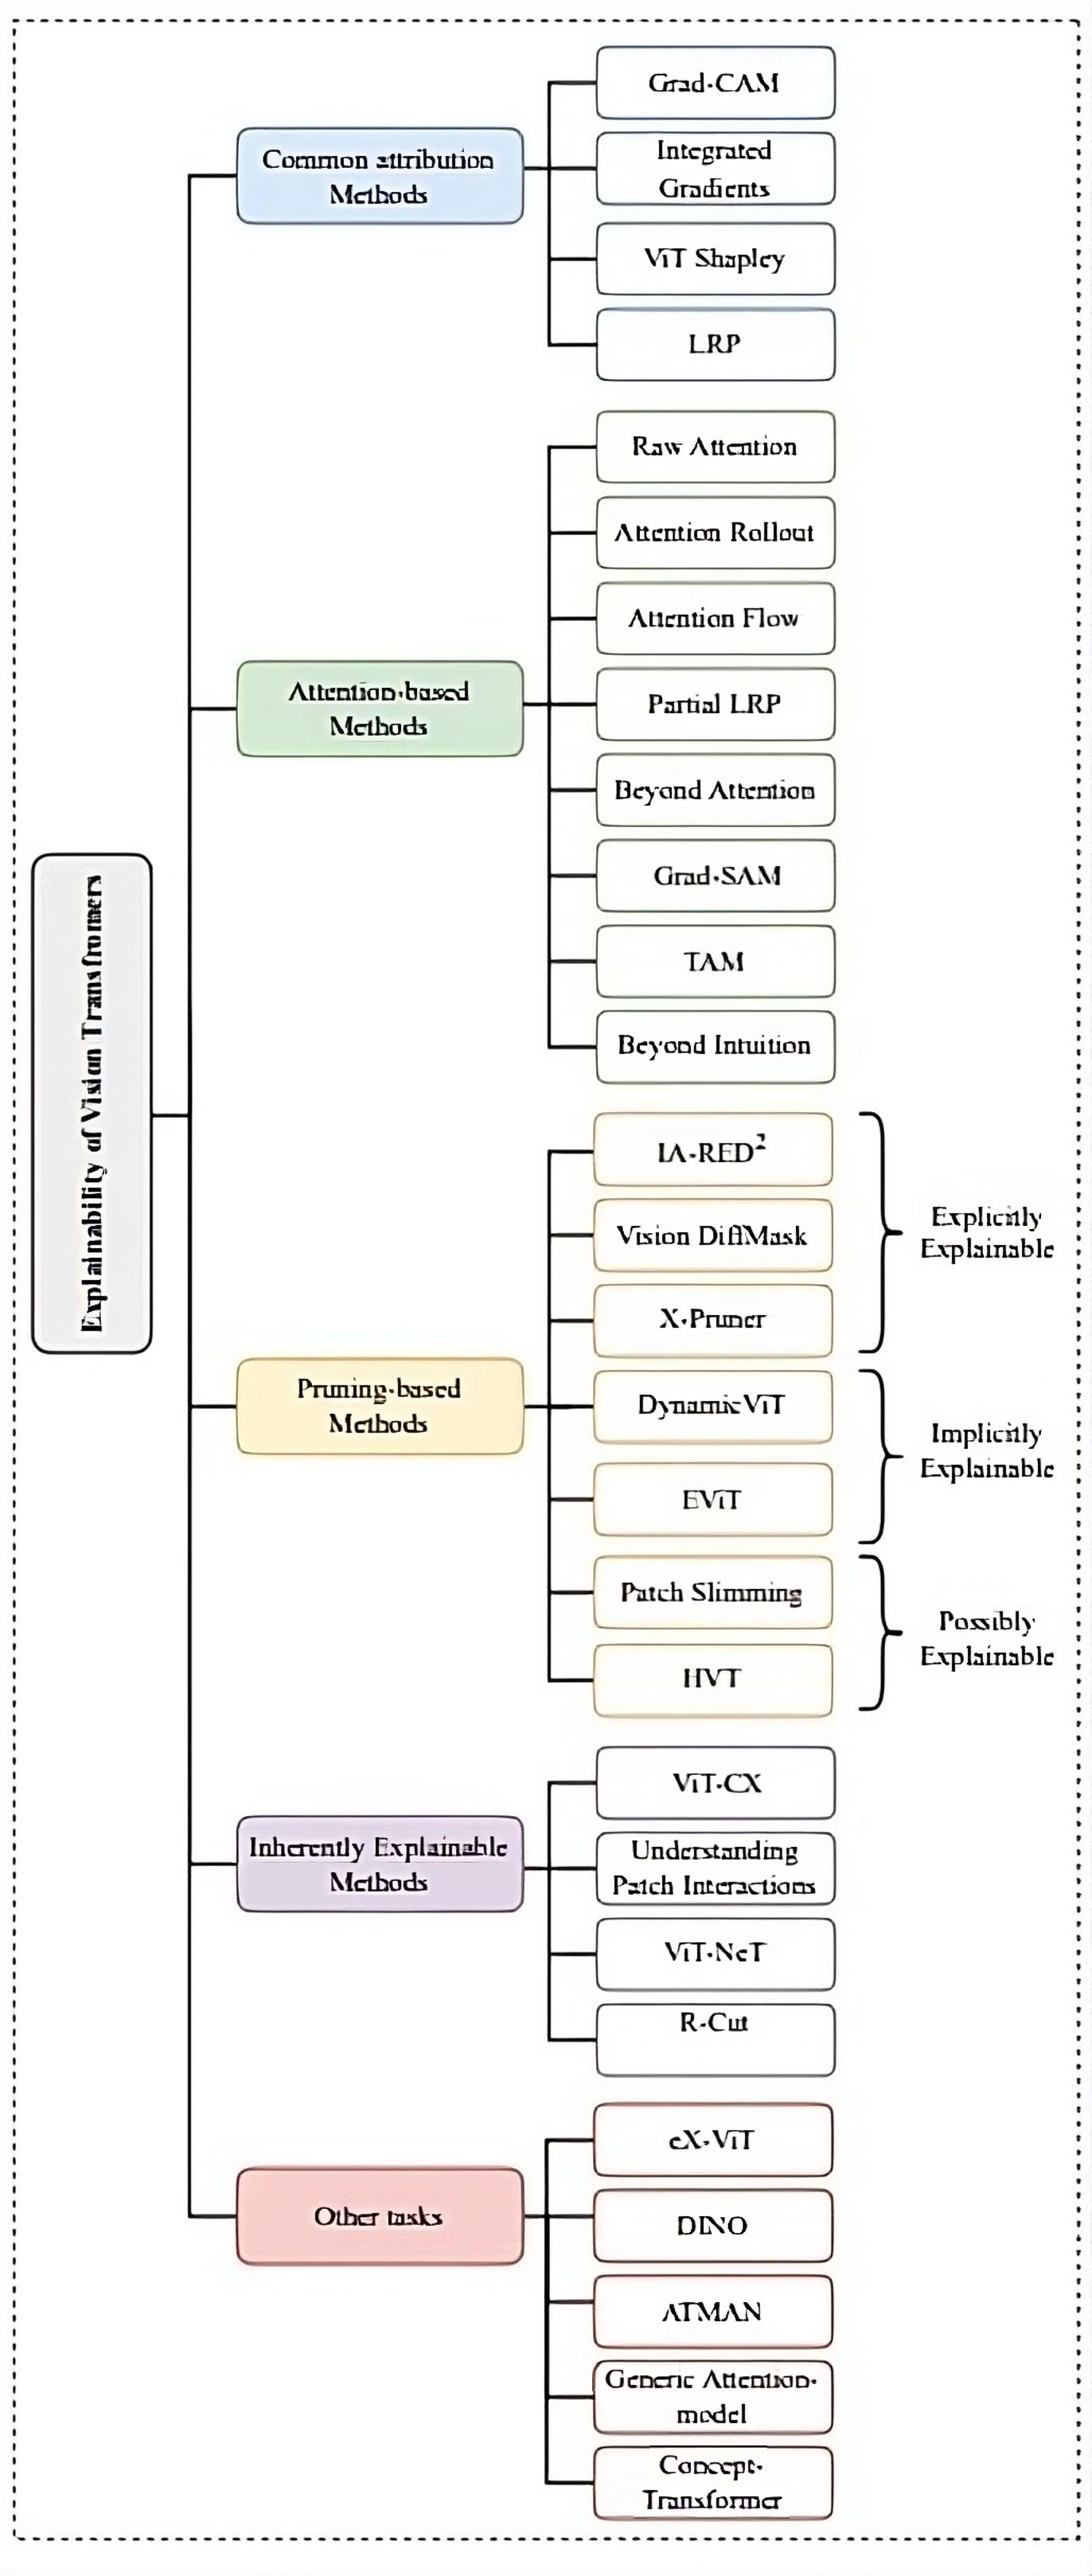
\includegraphics[width=0.6\textwidth]{2/figures/vt2.jpeg}
  		\caption{ Taxonomía de los métodos de explicabilidad para
  			Transformadores de visión (\cite{tecnica1})}
  	\end{center}
  \end{figure}
  
   \subsubsection{ Métodos basados en atención}
  Los métodos basados en atención aprovechan el mecanismo de atención de los modelos para identificar y priorizar las partes más relevantes de una secuencia de entrada. Muchos enfoques existentes se centran en utilizar los pesos de atención o el conocimiento codificado en ellos para explicar el comportamiento del modelo. En aplicaciones basadas en visión, la visualización de los pesos de atención puede ser útil para identificar patrones de atención, aunque puede volverse menos confiable a medida que la red crece más profunda y más compleja. Para superar estos desafíos, se han introducido dos métodos: "Attention Rollout" y "Attention Flow", que cuantifican el flujo de información y aproximan la atención a los tokens de entrada de manera más holística. Estos métodos tienen sus limitaciones, por lo que se han desarrollado enfoques adicionales, como "GradSAM" y "Transition Attention Maps" (TAM), que aplican funciones como gradientes a los pesos de atención para mejorar la explicación de las predicciones del modelo. Además, el marco "Beyond Intuition" propone una aproximación novedosa para aproximarse a las contribuciones de los tokens, operando en dos etapas: percepción de atención y retroalimentación de razonamiento.
  
     \begin{figure}[H]
  	\begin{center}
  		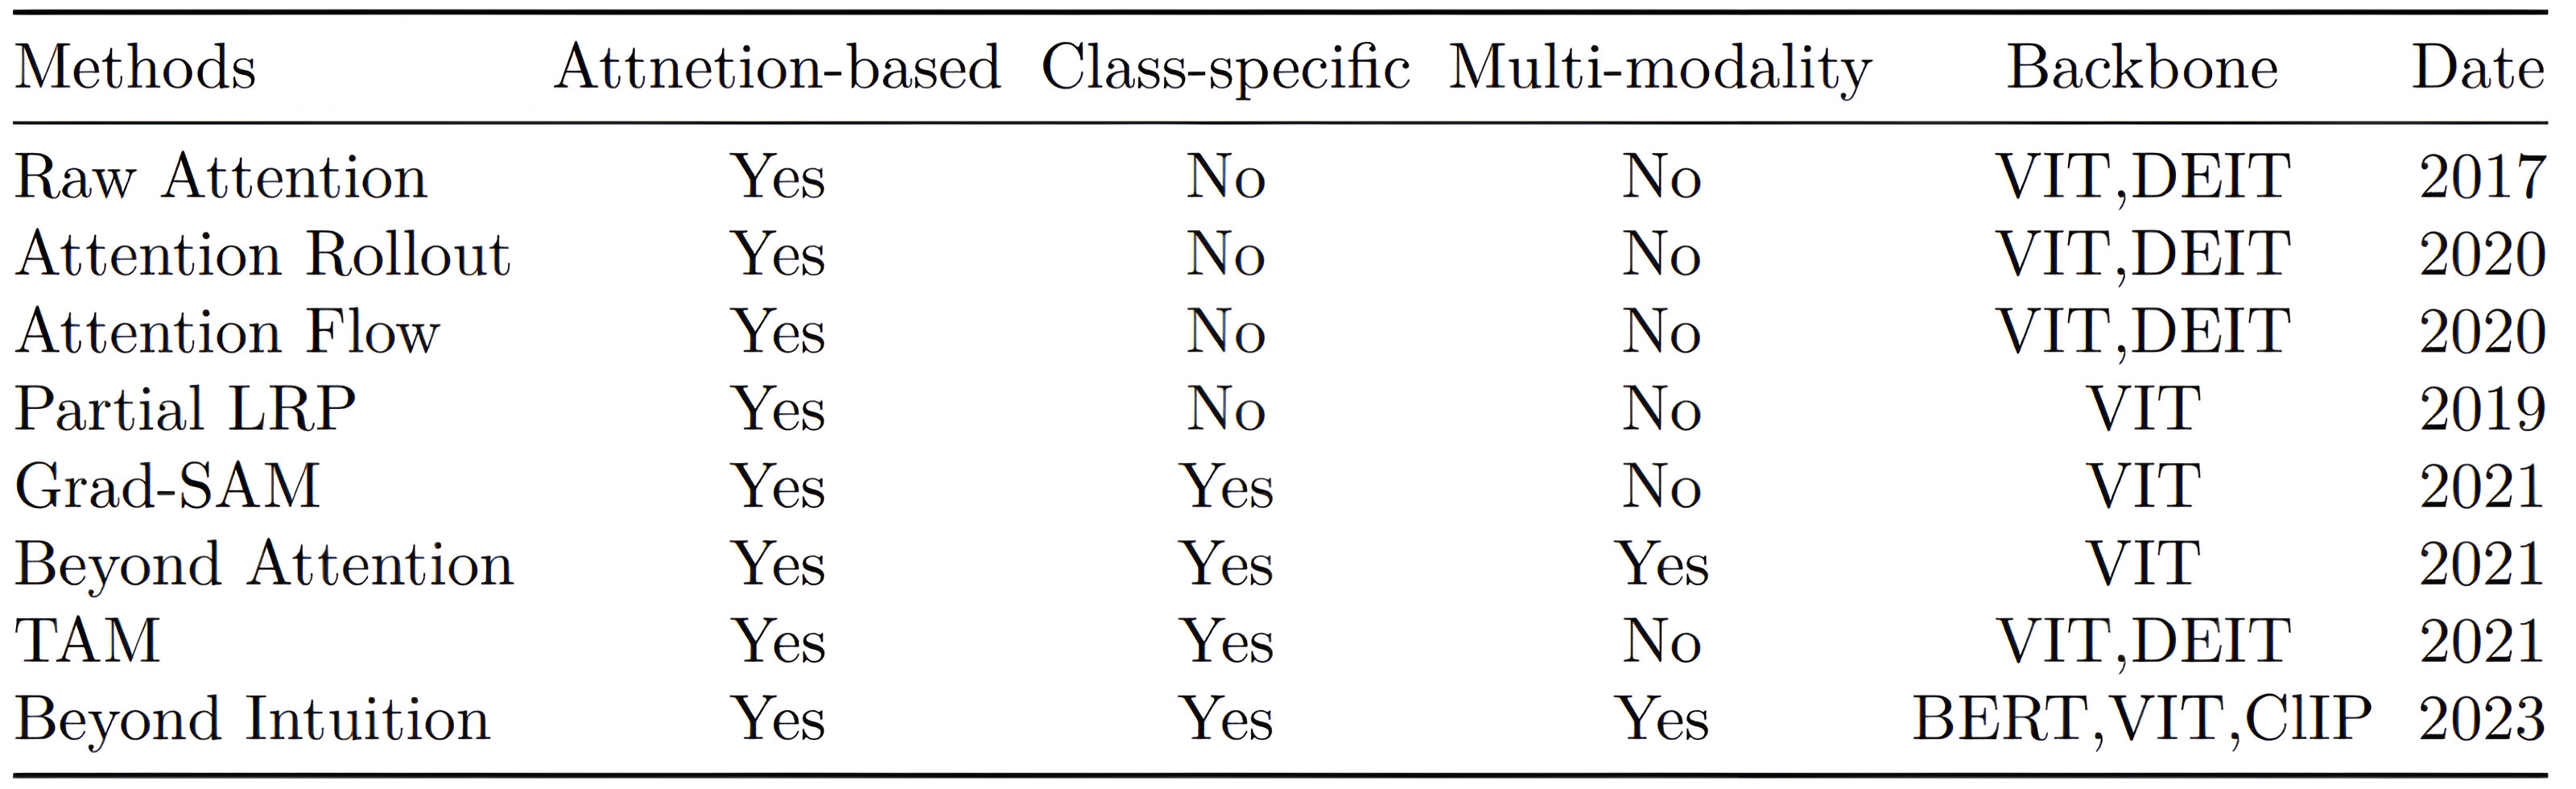
\includegraphics[width=1\textwidth]{2/figures/vt3.jpeg}
  		\caption{ Comparación de los métodos basados en atención desde diferentes perspectivas (\cite{tecnica1})}
  	\end{center}
  \end{figure}
  
       \begin{figure}[H]
  	\begin{center}
  		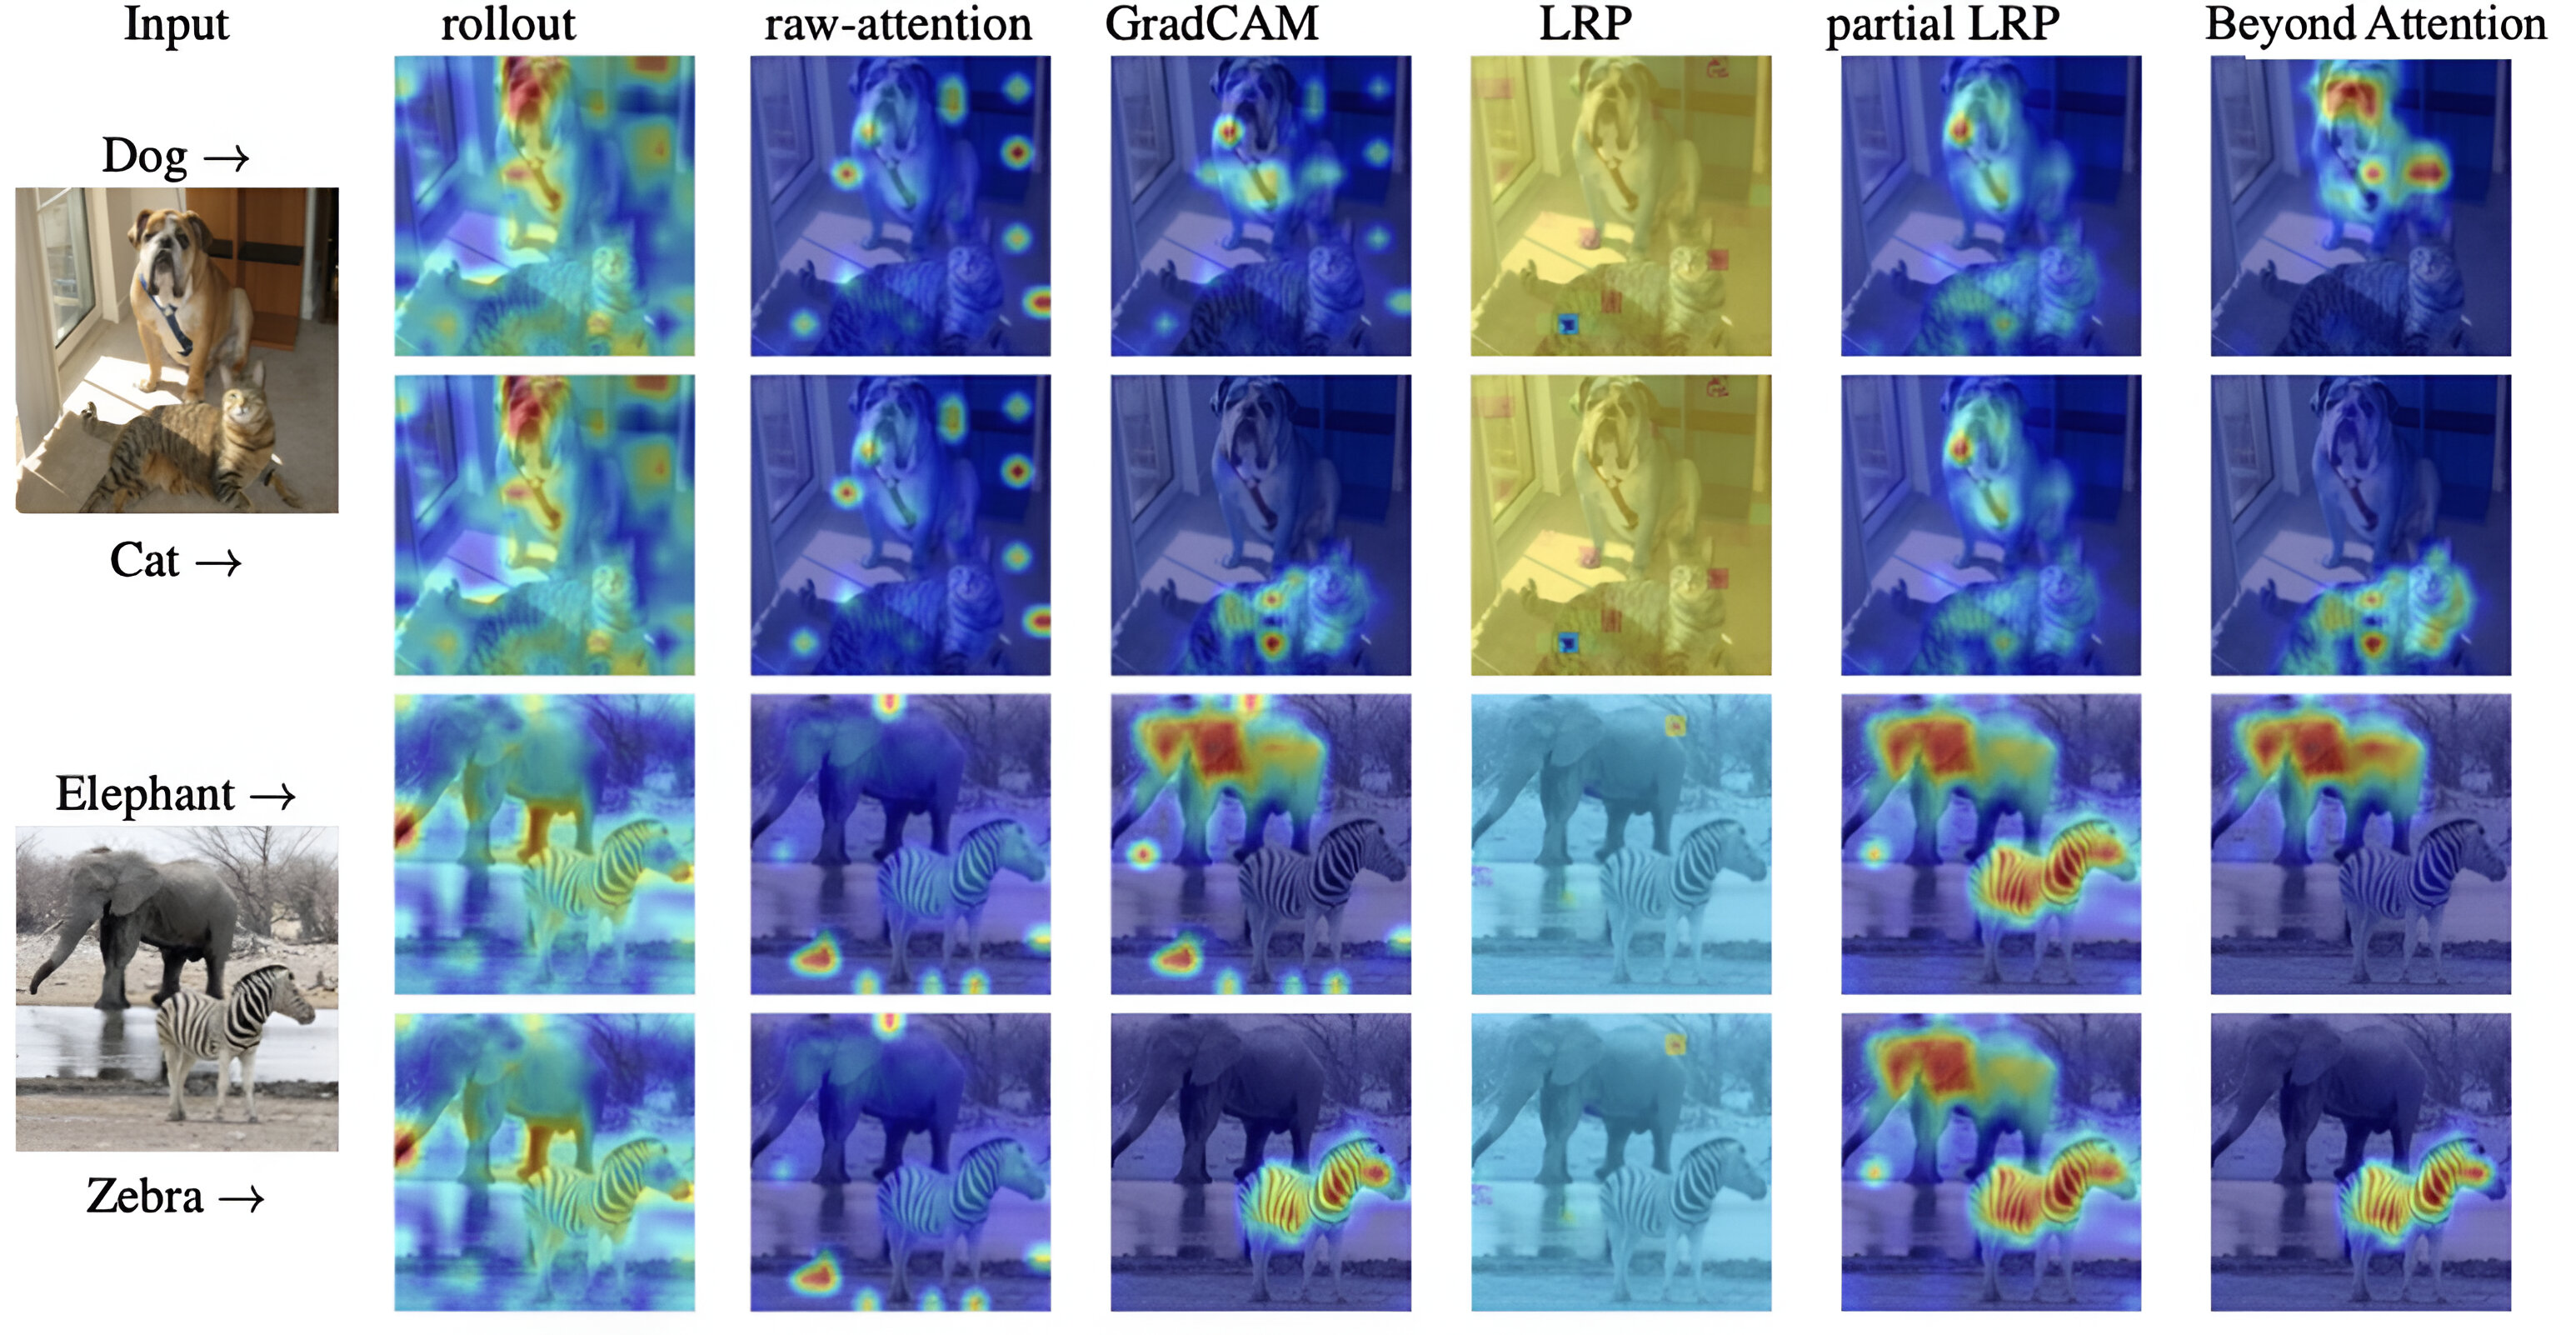
\includegraphics[width=1\textwidth]{2/figures/vt4.jpeg}
  		\caption{ Visualizaciones específicas de clase de varios métodos basados en la atención, para cada imagen se pueden ver resultados de dos clases diferentes(\cite{tecnica1})}
  	\end{center}
  \end{figure}
  
\subsubsection{ Métodos basados en la poda} 
Los métodos basados en poda son una poderosa herramienta utilizada para optimizar la eficiencia y complejidad de los transformers. Estos métodos intentan eliminar elementos redundantes o poco informativos como tokens, parches, bloques o cabezas de atención de las redes. Algunos de estos métodos están explícitamente desarrollados con fines de explicabilidad, mientras que otros se centran principalmente en mejorar la eficiencia y no tienen como objetivo específico la explicabilidad. Sin embargo, estudios indican que las técnicas del segundo grupo también pueden impactar positivamente la explicabilidad del modelo. Se pueden categorizar los métodos de poda basados en ViT en tres grupos: métodos explícitamente explicables, implícitamente explicables y posiblemente explicables.

Entre los métodos de poda explícitamente explicables, hay varios enfoques notables que buscan proporcionar modelos menos complejos y más interpretables. Por ejemplo, el método IA-RED2 busca encontrar el equilibrio perfecto entre eficiencia e interpretabilidad al eliminar dinámicamente los parches menos informativos, lo que resulta en una velocidad significativamente mayor con una pérdida mínima de precisión. Otro método, X-Pruner, está diseñado específicamente para podar unidades menos significativas, logrando importantes ahorros computacionales sin perder precisión.

Por otro lado, los métodos de poda implícitamente explicables, como el marco DynamicViT, están diseñados principalmente para mejorar la eficiencia de la red, pero también pueden mejorar la explicabilidad al localizar las partes críticas de la imagen que contribuyen más a la clasificación. EViT es otro enfoque innovador que reorganiza los tokens de una imagen basándose en el concepto de atención, manteniendo los tokens más relevantes mientras fusiona los menos atentos en un solo token, lo que reduce los costos computacionales sin comprometer la precisión del modelo. Estos métodos mejoran la interpretabilidad y ofrecen una comprensión más clara de las decisiones del modelo.   

   \begin{figure}[H]
	\begin{center}
		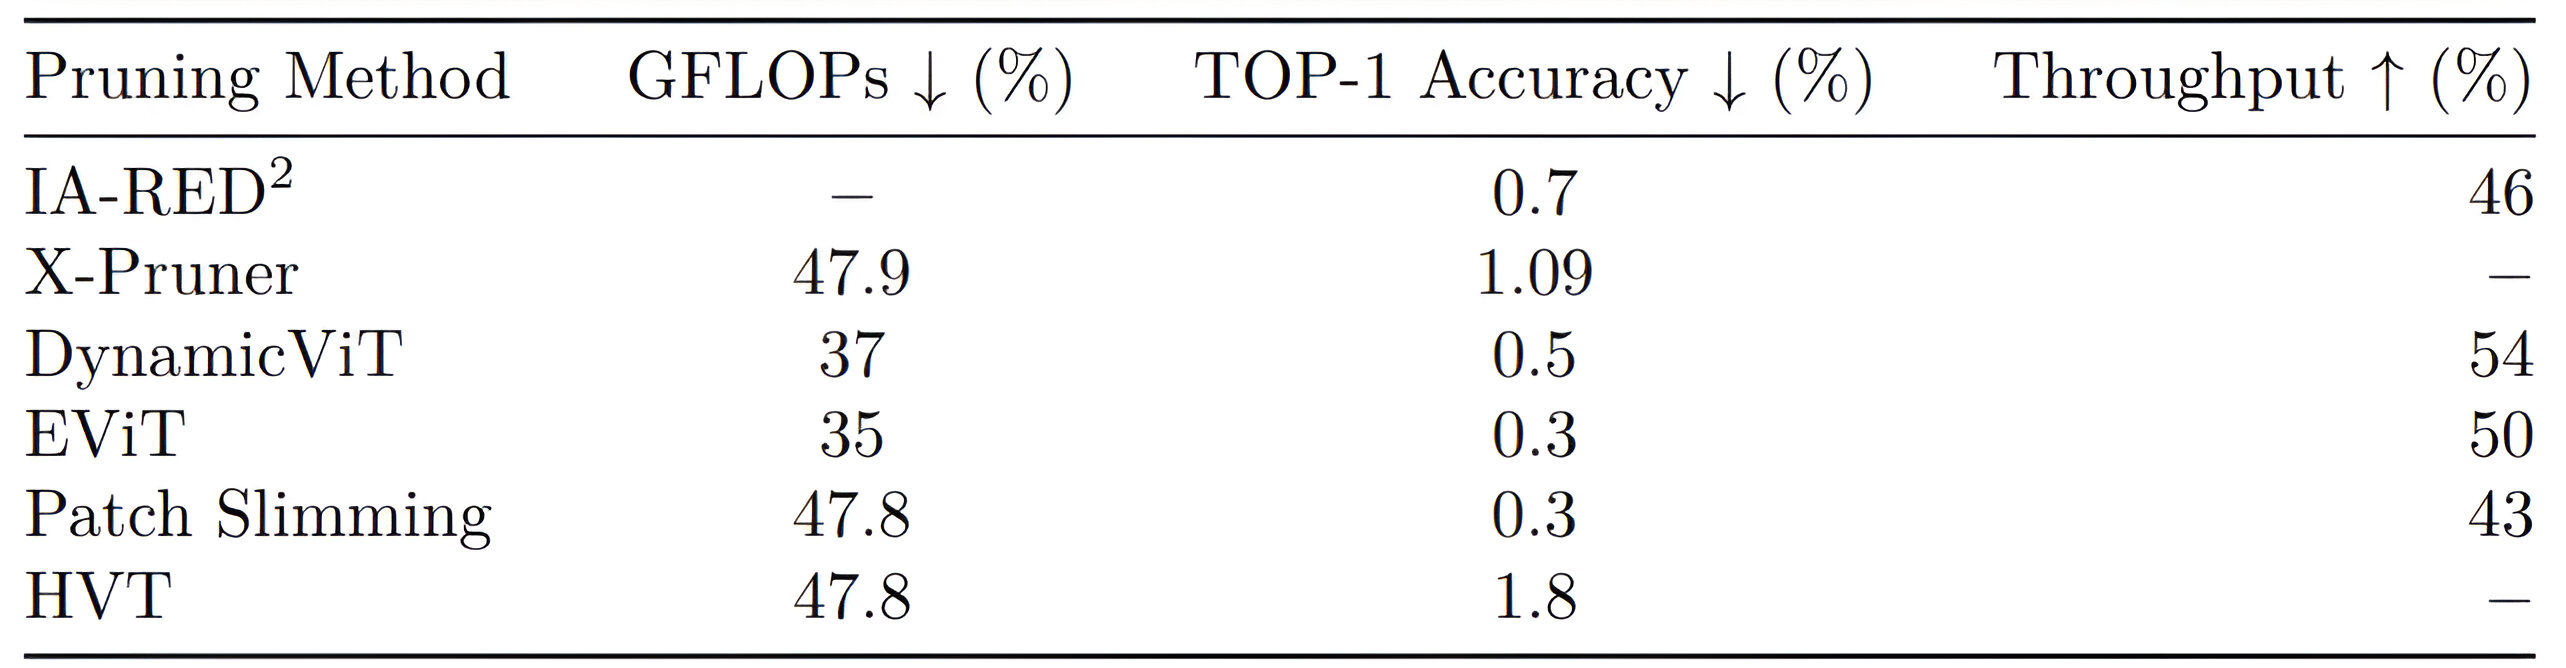
\includegraphics[width=1\textwidth]{2/figures/vt5.jpeg}
		\caption{Comparación de diferentes métodos basados en la poda aplicados a DeiT-S en el conjunto de datos ImageNet(\cite{tecnica1})}
	\end{center}
\end{figure}


Los métodos posiblemente explicables son enfoques adicionales de poda que, aunque inicialmente no se diseñaron para mejorar la interpretabilidad de ViT, podrían ofrecer un potencial para investigar su impacto en la explicabilidad de los modelos. Por ejemplo, Patch Slimming es un algoritmo novedoso que acelera ViTs al dirigirse a los parches redundantes en las imágenes de entrada, lo que potencialmente destaca características visuales importantes y mejora la interpretabilidad. Otro enfoque, Hierarchical Visual Transformer (HVT), mejora la escalabilidad y el rendimiento de ViTs al reducir gradualmente la longitud de la secuencia a medida que aumenta la profundidad del modelo. Aunque estos métodos se han evaluado principalmente en términos de eficiencia, existe una brecha significativa en la literatura en cuanto a la evaluación de su explicabilidad. En contraste, los métodos inherentemente explicables, como ViT-CX, se centran en desarrollar modelos que puedan explicarse a sí mismos, utilizando herramientas interpretables como mapas de saliencia para proporcionar explicaciones más significativas.

   \begin{figure}[H]
	\begin{center}
		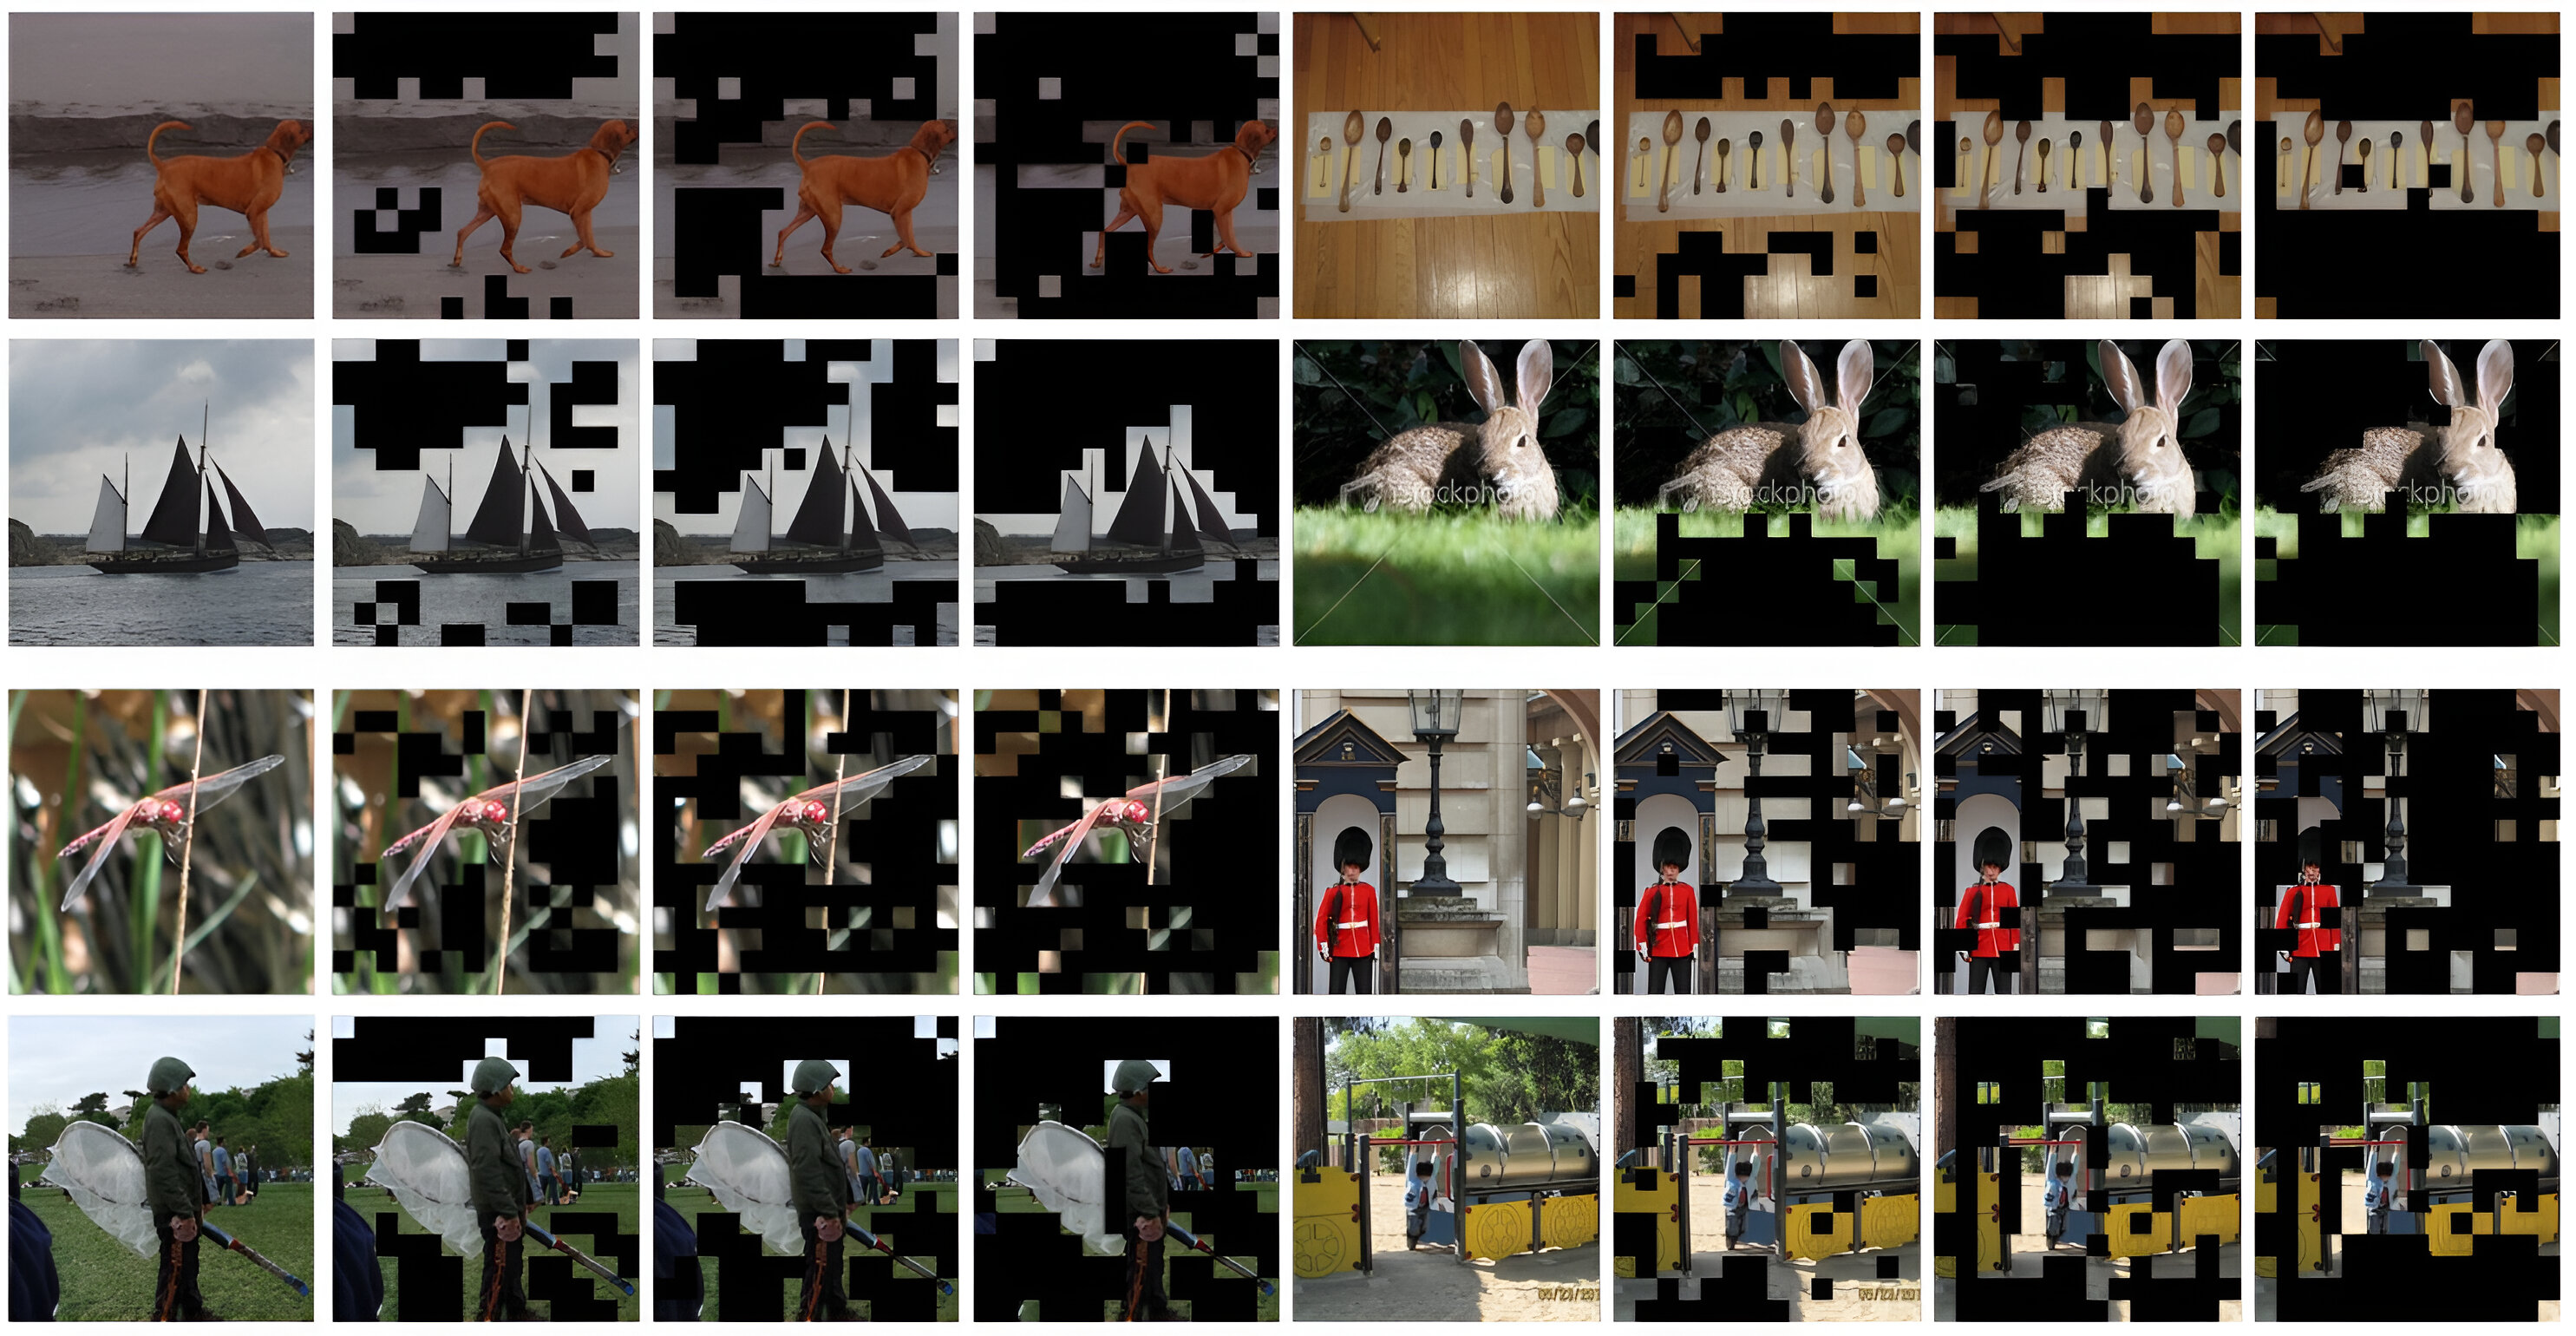
\includegraphics[width=1\textwidth]{2/figures/vt6.jpeg}
		\caption{Visualización de tokens desatentos en EViT-DeiT-S con 12 capas; Se puede ver que las fichas de falta de atención se fusionan gradualmente (como se representa mediante áreas enmascaradas) o se eliminan, mientras que las fichas más informativas se conservan. Esto permite a los ViT centrarse en tokens específicos de clase en imágenes, lo que conduce a una mejor interpretabilidad(\cite{tecnica1})}
	\end{center}
\end{figure}


 \subsubsection{Evaluación de explicación}
 En secciones anteriores, presentamos varias técnicas de explicación desarrolladas específicamente para aplicaciones basadas en ViT. Sin embargo, evaluar qué tan bien estas técnicas representan el proceso de razonamiento de un modelo presenta diferentes desafíos. Para abordar esta preocupación, la literatura sugiere una serie de criterios evaluativos, que ayudan a seleccionar y diseñar la técnica de explicabilidad más apropiada. A continuación, se resumen estos criterios:
 \begin{itemize}
 	\item \textbf{Deletion and Insertion:} Se utilizan para evaluar la fidelidad de un mapa de saliencia al modelo objetivo. Calculan cómo el mapa de saliencia identifica los píxeles más influyentes para la predicción del modelo.
 	\item \textbf{Effective Complexity:} Evalúa el número de atribuciones que superan un umbral, indicando la importancia o insignificancia de las características correspondientes.
 	
 	\item \textbf{Faithfulness:} Método para evaluar la calidad de las atribuciones de características sin intervención humana, midiendo cuán precisamente las atribuciones de características se alinean o correlacionan con las predicciones del modelo.
 	
 	\item \textbf{(In)fidelity:} Se utiliza para evaluar qué tan bien una explicación captura los cambios en las predicciones de un modelo cuando la entrada sufre perturbaciones significativas.
 	
 	\item \textbf{Intersection over Union (IoU) test:} Métrica estándar para evaluar el rendimiento de los detectores y seguidores de objetos, que también se ha utilizado para evaluar métodos de explicabilidad midiendo la superposición entre los mapas de explicabilidad predichos y las cajas delimitadoras de la verdad terrenal de los objetos de interés.
 	
 	\item \textbf{Perturbation Tests:} Funcionan al enmascarar gradualmente tokens de entrada basándose en las explicaciones proporcionadas por el método de explicabilidad dado.
 	
 	\item \textbf{Pointing Game:} Método para evaluar los mapas de saliencia de la explicación en comparación con las cajas delimitadoras anotadas por humanos.
 	
 	\item \textbf{Segmentation Tests:} Consideran cada visualización como una segmentación suave de la imagen y las comparan con la verdad terrenal proporcionada en el conjunto de datos.
 	
 	\item \textbf{Sensitivity:} Evalúa cómo varían las explicaciones con pequeñas perturbaciones en la entrada.
 	
 	\item \textbf{Sensitivity-n:} Propuesto para probar valores de atribución específicos en lugar de considerar solo las clasificaciones de importancia.
 \end{itemize}
 
    \begin{figure}[H]
 	\begin{center}
 		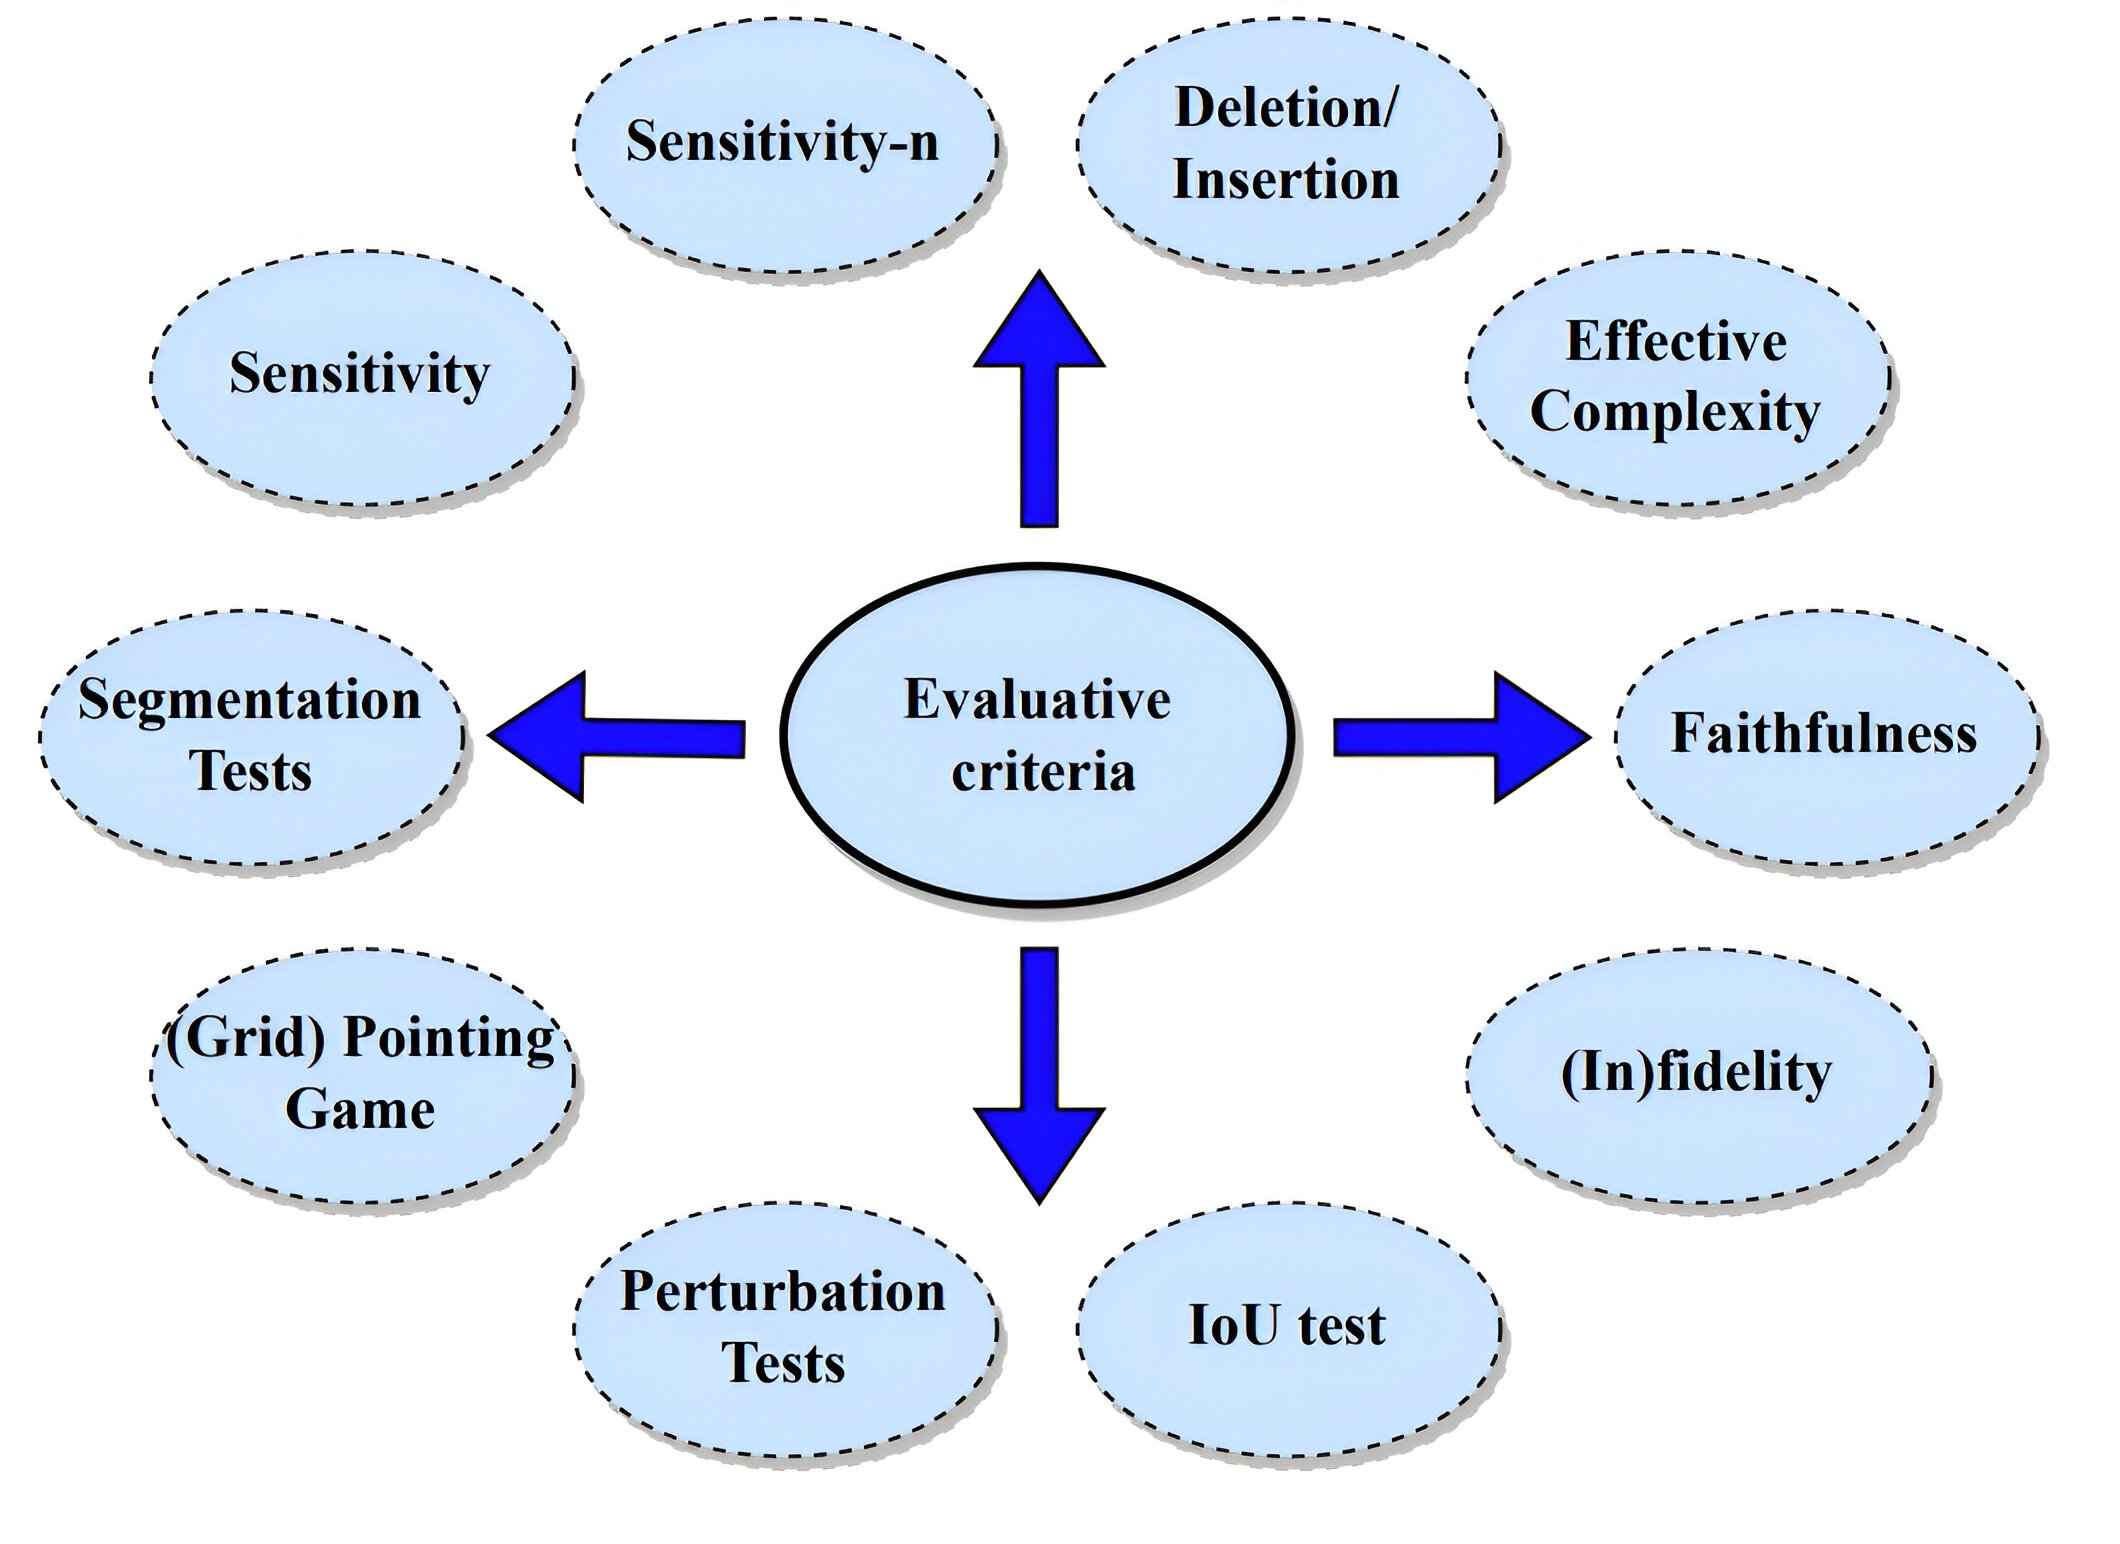
\includegraphics[width=1\textwidth]{2/figures/vt8.jpeg}
 		\caption{Diferentes criterios para evaluar los métodos de explicabilidad en aplicaciones basadas en la visiónt(\cite{tecnica1})}
 	\end{center}
 	\end{figure}
 		
 \subsubsection{Conclusión}
 
 En resumen, este trabajo ofrece una visión completa de las técnicas de explicabilidad propuestas para los transformers visuales. Hemos proporcionado una taxonomía de los métodos basada en sus motivaciones, estructuras y escenarios de aplicación, categorizándolos en cinco grupos. Además, detallamos los criterios de evaluación de la explicabilidad, así como las herramientas y marcos de trabajo utilizados. Por último, discutimos varios problemas esenciales pero poco explorados para mejorar la explicabilidad de los transformers visuales y sugerimos direcciones de investigación potenciales para futuras inversiones. Esperamos que este artículo de revisión ayude a los lectores a comprender mejor los mecanismos internos de los transformers visuales, así como a resaltar problemas abiertos para trabajos futuros.
 \subsection{Redes neuronales convolucionales}
 
 \subsection{You Only Look One (YOLO)}
 
 \subsection{Support Vector Machine}
 
 
 